\documentclass[12pt,twoside]{article}
\newcommand\tab[1][1cm]{\hspace*{#1}}
\usepackage{pdfpages}
\usepackage[utf8]{inputenc}
\usepackage{graphicx}
\pagenumbering{roman}
\begin{document}


\includepdf[pages=-3]{CSE496_111044040_ProjectReport.pdf}
\mbox{}
\thispagestyle{empty}
\newpage

\includepdf[pages=-]{Jury.pdf}
\mbox{}
\thispagestyle{empty}
\newpage
\addcontentsline{toc}{section}{PREFACE}
\section*{PREFACE} 
I would like to express my sincere thanks to who contributed to preparation of the
first draft and Dear Asst. Prof. Dr. Zafeirakis ZAFEIRAKOPOULOS and Gebze Technical University for supporting this work.
I also give my full respect and love to my family for supporting me during the every
aspect of education life.\newline \newline \newline
\textbf{May, 2017} \tab[7.5cm]
\textbf{Yunus Emre AVCI}


\newpage

\tableofcontents

\newpage
\listoffigures
\newpage
\addcontentsline{toc}{section}{SUMMARY}
\section*{SUMMARY}
Two notions of polytope volume were combined in this project, namely the
Euclidean volume and the discrete volume. The Euclidean volume is the classical
notion of volume, while the discrete volume is the number of integral points in the
polytope. For a cube, in a cube of side 2, the Euclidean volume is 2 3 = 8 and the
discrete volume is 27.\newline \newline
Emiris – Fisikopoulos' fast algorithms were used to approximate the Euclidean
volume(note that exact computation of volume is \#P hard), and were combined with Ehrhart Theory to compute the discrete volume. The polytope specified by the
integer values in the file with extension .ine is read, and rewritten to a file which is a new dilated polytope. The volume approximation determines the upper and lower
bounds of the new system. Binomial and monomial calculations are made with
dilated polytope and b and H values are determined. Linear programming creates a
file with lp extension to obtain H vector. The Ehrhart polynomial obtained using the
GLPK library and the discrete volume are found using LattE.\newline \newline
Emiris-Fisikopoulos' fast volume approximation that uses the CGAL library, have
been used for Euclidean volume. All steps were implemented as
aforementioned. The system has been tested with different types of polytopes such
as; cube, birkhoff, crosspolytope.
\newpage
\addcontentsline{toc}{section}{\"OZET}
\section*{\"OZET}
Polytope hacmi hesaplama için bulunan Öklid hacim ve ayrıt hacmi bu projede
birleştirildi. Öklid hacmi klasik hacim kavramı iken ayrıt hacmi, polytope'daki
integral noktalarının sayısıdır. Bir küp için kenar uzunluğu 2 ise Öklid hacmi 2 3 = 8
ve ayrıt hacim ise 27'dir.\newline \newline
Emiris-Fisikopoulos'un hızlı volume approximation algoritması, Öklid hacmi
yaklaşık olarak bulurken kesin sonucun bulunması \#P hard bir problemdir ve ayrıt
hacmi hesaplamak için Ehrhart teorisi ile birleştirildi. Uzantısı .ine olan dosyada
integer değerlerle belirtilen polytope okunur, dilate edilerek oluşan yeni polytope
dosyaya tekrar yazılır. Volume approximation uygulanarak yeni sistemin alt ve üst
sınırları belirlenir. Dilated polytope ile Binomial ve monomial hesabı yapılarak b ve
H değerleri belirlenir ve Lineer programlama ile H vektörü elde edilmek üzere lp
uzantılı dosya oluşturulur. GLPK kütüphanesi kullanılarak elde edilen Ehrhart
polynomial ile LattE kullanılarak discrete volume bulunur.\newline \newline
Cgal kütüphanesini içeren Emiris-Fisikopoulos'un hızlı hacim yaklaşımı öklid hacmi
için kullanılmıştır. Yukarıda bahsedilen tüm adımlar uygulanmıştır. Sistem, farklı
polytope türleri ile test edilmiştir; küp, birk, cross..
\newpage
\section{INTRODUCTION}
\pagenumbering{arabic}

\par
This report aims to show how to get discrete volume is related to
Euclidean volume and how the methods can be used naturally for various problems
of Euclidean and discrete volumes of polytopes.\newline
\par 
A fundamental problem in discrete and computational geometry is to
compute the volume of a convex body in general dimension or, more particularly, of
a polytope. In the past 15 years, randomized algorithms for this problem have
witnessed a remarkable progress. Starting with the breakthrough poly-time
algorithm for computing exactly the volume of a convex polytope given as the set of a finite system of linear inequalities. \newline
\par
Convex bodies are typically given by a membership oracle. A polytope $P \subseteq R^d$ can also be represented as the convex hull of vertices (V-polytope) or, as is the
case here, as the (bounded) intersection $P := \{ x \in R^d | Ax \leq b\} $ of m halfspaces
given by $A \in R^mxd $ , $b \in R m$ halfspaces (H-polytope); $\partial P$ is its boundary, and
$O^* (.)$ hides polylog factors in the argument. The input includes approximation factor
$\epsilon < \theta$. Volume computation is \#P hard for V- and for H-polytopes \cite{computeVolume}.\newline
\par
Several questions of sampling combinatorial structures such as contingency
tables and more generally lattice points in polytopes may be reduced to sampling a
polytope. No simple sampling method exists unless the body has standard shape,
e.g., simplex, cube or ellipsoid. Acceptance-rejection techniques are inefficient in
high dimensions. E.g., the number of uniform points one needs to generate in a
bounding box before finding one in P is exponential in d.\newline
\par

When is the volume of a convex polytope in R n close to the number of lattice points
in the polytope? It is shown if the polytope contains a ball of radius $n\sqrt{logm}$, where m is the number of facets, then the volume approximates the number of lattice
points to within a constant factor. This general condition is then specialized to
derive polynomial time sampling and counting algorithms for various combinatorial
problems whose solutions can be viewed as lattice points of convex polytopes[8].\newline \newline
\par
The reason of working with this subject was to have experience in this field
and to learn the tools I used to develop. Project goals, requirements, system
architecture, test results and working method are explained on the following parts.


\subsection{EHRHART THEORY}


There are two ways to define a general convex polytope in $R^n$ , the first being
the halfspace description. A halfspace in $R^n$ is the set of solutions to a linear
inequality of the form $Ax \leq b$ for some $A \in R^n$ , $b \in R$. Other definition is, an affine
subspace $A \subset R^n$ of dimension d is a translate by some fixed $y \in R^n $of a d-dimensional linear subspace of $R^n$ .\newline 
\par
An integral polytope has an associated Ehrhart polynomial that encodes the
relationship between the volume of a polytope and the number of integer points the
polytope contains.\newline
\par
Informally, if $P$ is a polytope, and $tP$ is the polytope formed by dilated $P$ by a
factor of $t$ in each dimension, then $L(P, t)$ is the number of integer lattice points in $tP$.\newline
\par
More formally, consider a lattice L in Euclidean space $R^n$ and a d-
dimensional polytope P in $R^n$ with the property that all vertices of the polytope are points of the lattice. (A common example is $L=Z^n$ and a polytope for which all
vertices have integer coordinates.) For any positive integer $t$, let $tP$ be the t-fold dilation of P (the polytope formed by multiplying each vertex coordinate, in a basis for the lattice, by a factor of t), and let $ L(P,t) = \#(tP \cap L)$ be the number of lattice
points contained in the polytope $tP$. L is a rational polynomial of degree $d$ in $t$, i.e. there exist rational numbers $a_0 ... a_d$ such that: $L(P,t) = a^dt_d + a^{d-1}t_{d-1} + ... + a^0$ . Let
P be a d-dimensional unit hypercube whose vertices are the integer lattice points all
of whose coordinates are $0$ or $1$. In terms of inequalities
\[ P = \{ x \in Q^d : 0 \leq x i \leq 1; 1 \leq i \leq d \} \]
\newpage
\par
Then the $t$ dilation of $P$ is a cube with side length $t$, containing $ (t+1) d$
integer points. That is the ehrhart polynomial of the hypercube is $ L(P,t) = (t + 1) d$.
\newline
\par
Let P be a rational polytope. In other words, suppose $P = { x \in Q^d : Ax \leq b}$,
where $A \in R^{kxd}$ and $b \in Z^k$ .Then define $L(P,t) = \#({x \in Z^n : Ax \leq tb})$. In this case
$L(P,t)$ is a quasi-polynomial which is a generalization of polynomial.\newline
\par
Below figures are showing the lattice points according to intersection of
halfspaces with $t$ values.
\newline
\begin{figure}[!h]
  \centering
          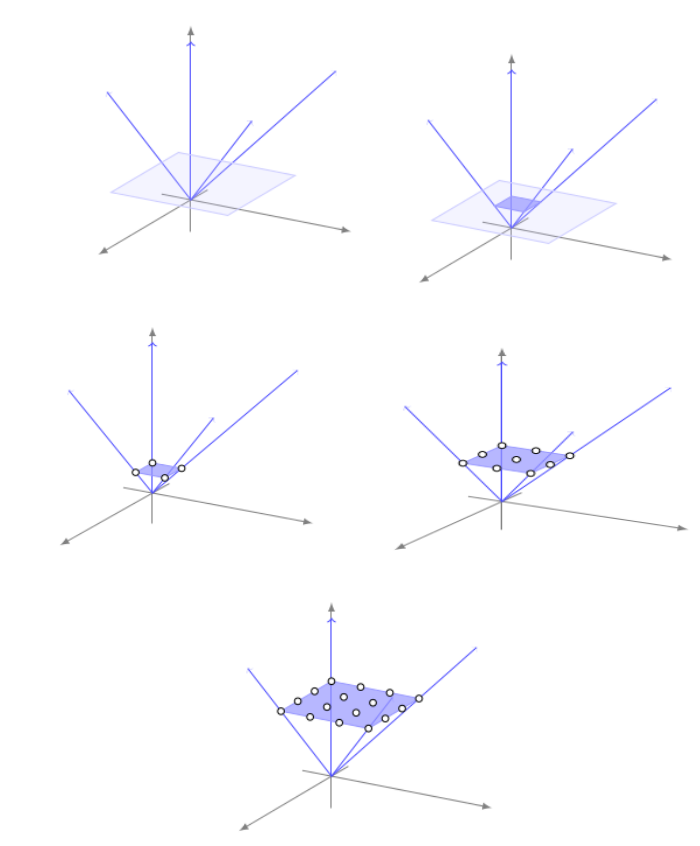
\includegraphics[width=0.65\textwidth]{tandlattice.png}
  \caption{t dilate values and their lattice point numbers}
\end{figure}


\newpage
\begin{figure}[t]
  \centering
          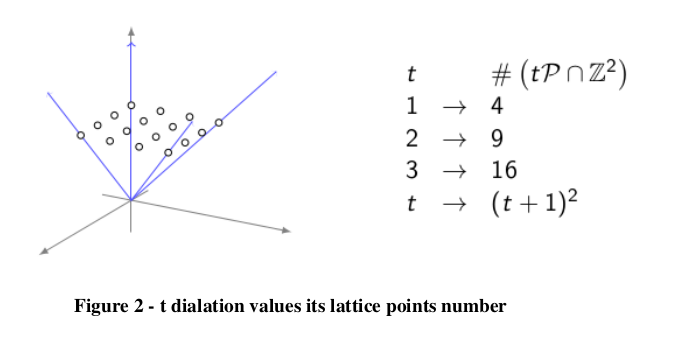
\includegraphics[width=0.65\textwidth]{tdialatevaleq.png}
  \caption{t dialation values its lattice points number and general equation}
\end{figure}

\subsection{INTERPOLATION}
\par
Let's assume $Lp(t)$ is a polynomial and $Lp(t) = at^2 + bt + 1$
\[ Lp_2(1) = a + b + 1 = 9,\]
\[ Lp_2(2) = 4a + 3b + 1 = 25,\]
linear system can be found from these two equalities so that $a = 4$ and $b = 4$.\newline
\par 
The volume can be approximated fast with $\in$ tolerance
\[(1- \in)vol(p) \leq Lp(t) \leq (1 + \in)Vol(p).\]
\par
If the bounds of the this equation are obtained from volume
approximation code results, and $t$ dilate value of polytope combined, we can get
\[t^d \mu_\in vol(p) \leq Lp(t) \leq t^d \mu_\in(t)vol(p).\]
\par
We can take each inequality pair from $	m\in(t)V_A(tP) \leq Lp(t) \leq N_\in(t)V_A(tP)$ then
draw $Lp(t) = \sum\limits_{i=0}^d  a_it^i$ values can be in scanned area. The coefficient vector of
$Lp(t)$ is a lattice point in $R^{d+1}$ . In particular, it is in the polytope I defined by the
inequalities: \newline

\[x_i \geq 0\]
\[ \sum\limits_{i=0}^d x_i{{t +d – i}\choose{d}} \geq m \]
\[ \sum\limits_{i=0}^d -x_i {{t +d – i}\choose{d}}  \geq -M\]
\par
Every polynomial can be written in monomial basis $\sum\limits_{i=0}^d  a_it^i$ in the monomial
basis $1,t,t^2 ,t^3 .. t^d$

\textit{Binomial Basis;} \newline
\par
Every polynomial of degree $d$ is a linear combinations of binomials. Let's give a
monomial – binomial conversion. Let $d$ be 2, we have unit square $P$ and monomial
equation is $Lp(t) = t^2 + 2t + 1$ \newline
\par
To get binomial of it $Lp(t) = \sum\limits_{j=0}^d h_j{{t + d -j}\choose {d}}$ then $h_j$ elements of $N$
description is used,
\[ b_0 = {{t + 2}\choose {2}} = \frac{(t+2)!}{t! 2!} = \frac{t^2 + 3t +2}{2}\]
\[ b_1 = {{t + 2 -1 }\choose {2}} = \frac{(t+1)!}{(t - 1)! 2!} = \frac{t^2 + t}{2}\]
\[ b_2 = {{t + 2 - 2}\choose {2}} = \frac{t!}{(t-2)! 2!} = \frac{t^2 -t}{2}\]
\[ Lp(t) = h_0b_ 0 + h_1b_1 + h_2b_2 \]
\[ Lp(t) = t^2 /2 (h_0 + h_1 + h_2 ) + t/2 (2h_0 + h_1 – h_2 ) + 1/2(h_0 )\]
\par
After $b_0 ,b_1 ,b_2$ equations we should ask how to get the monomial equivalent
that is $t^2 + 2t + 1$. So that binomial equation should be $Lp(t) = b_0 + b_1.$ If we have a
triangle, our binomial equation could be $Lp(t) = b_0.$ \newline

\begin{figure}[!h]
  \centering
          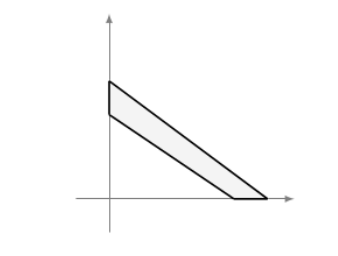
\includegraphics[width=0.30\textwidth]{scannedarea.png}
  \caption{scanned area of inequalities to search points}
\end{figure}
\newpage
\par
Let assume t be 4 \newline
\[ 12 \leq h_0b_0 + h_1b_1 + h_2b_2 \leq 16\]
$ b_0(4) = 15 , b_1(4) = 10, b_2(4) = 4$ these are successful coefficients.\newline
$23 \leq 15 h_0 + 10h_1 + 4h_2 \leq 26$ which we know that h's are nonnegative so we
can draw with half spaces.\newline
\par
If initially polynomial degree d then we have d+1 dimension in monomial basis and binomial basis.
${15X + 10y + 4z \leq 26 , 23 \leq 15x+ 10y + 4z }$ candidate h-vector of this
inequalities can be $(1,1,0)$ etc.
\newline
\subsection{PROJECT DEFINITION}
\par
Explore the use of continuous, Euclidean, volume for the computation of
discrete volume. The Euclidean volume is calculated using volume
approximation and is combined with Ehrhart polynomial and finally discrete
volume has been calculated. The Flow chart of the project is shown below. \newline
\begin{figure}[!h]
  \centering
          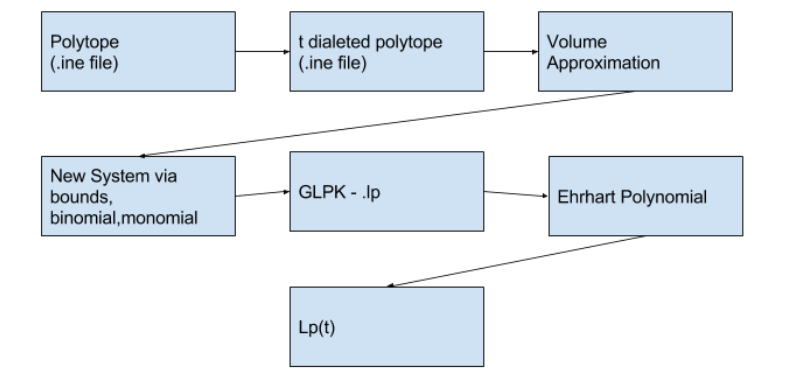
\includegraphics[width=0.70\textwidth]{flowchart.png}
  \caption{flowchart of the system}
\end{figure}
\newline
\newpage
Given an inequality file with different types of polytopes such that
\begin{figure}[!h]
  \centering
          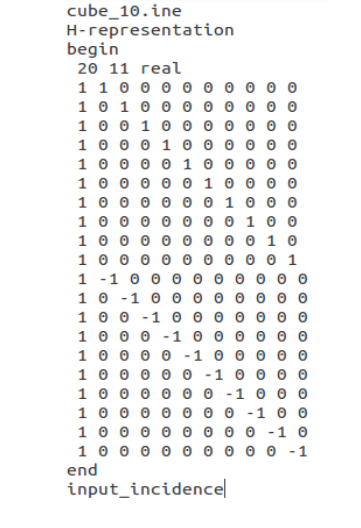
\includegraphics[width=0.40\textwidth]{sampleine.png}
  \caption{sample .ine file, cube10.ine}
\end{figure}


\par
The input file is d-dimensional enumerated polytope whose dimension can be
determined by looking for fourth rows first number. Polytope can be dialate with t
times. New dilated file is created. To compute fast and find euclidean volume the
volume approximation is used.\newline
\par
Bounds are got from result of Emiris-Fisikopoulos' approximation result.
Bounds are shown below with bold characters.\newline
\par 
Experiment 1 \newline
10 20 10 0 1 [0,0] 9210 11 9.948861e+12 \textbf{ [9.948861e+12,9.948861e+12]} 0 - inf 0 0.267046 0.000375
\newline
\par
Monomial – binomial conversion is applyied for the linear programming
with GLPK. In order to determine $Lp(t)$ discerete volume LattE is used over Ehrhart polynomial
\section{PROJECT REQUIREMENTS}

Project requirements have been listed below for volumes of polytopes: \newline
\begin{itemize}
	\item Perform a large number of experiments for Ehrhart polynomial computation
	\item Approximate the Euclidean volume using fast algorithms
	\begin{itemize}
		\item Emiris-Fisikopoulos code is finding the euclidean volume of polytopes. It uses CGAL library and it's written on C++.
	\end{itemize}
	\item Use CGAL and Emiris – Fisikopoulos code for volume approximation
	\item To get bounds for ehrhart polynomial and to find euclidean volume of polytopes
	\item Combine fast volume algorithms with Ehrhart Theory
	\begin{itemize}
		\item Bounds that were found in result of fast volume algorithms and
monomial and binomial basis are using for Ehrhart Theory to get
candidate volume.

	\end{itemize}
	\item Compute discrete volume
	\end{itemize} 
\par	
	Project has many tools for realizing this requirements. Those are listed and
explained below.
\begin{itemize}
	\item Docker
	\begin{itemize}
		\item Docker is a tool designed to make it easier to create, deploy, and run
applications by using containers. Containers allow a developer to
package up an application with all of the parts it needs, such as
libraries and other dependencies, and ship it all out as one package.
By doing so, thanks to the container, the developer can rest assured
that the application will run on any other Linux machine regardless
of any customized settings that machine might have that could differ
from the machine used for writing and testing the code. For the
installation in Linux machine sudo apt-get install docker.io command
can be used. After install step to check installation give the sudo
dokcer hello world command to command line
	\end{itemize}
	\item CGAL library
	\begin{itemize}
		\item CGAL is a software project that provides easy access to efficient and
reliable geometric algorithms in the form of a C++ library. CGAL is
used in various areas needing geometric computation, such as
geographic information systems, computer aided design, molecular
biology, medical imaging, computer graphics, and robotics.
	\end{itemize}
	\item Python
	\begin{itemize}
		\item NumPy \newline 
		\par 
		NumPy is the fundamental package for scientific computing
with Python. It contains among other things a powerful N-
dimensional array object sophisticated (broadcasting) functions tools
for integrating C/C++ and Fortran code useful linear algebra, Fourier
transform, and random number capabilities
		\item SymPy \newline
		\par
		SymPy is a Python library for symbolic computation. It
provides computer algebra capabilities either as a standalone
application, as a library to other applications. SymPy is trivial to
install and to inspect because it is written entirely in Python
with few dependencies. This ease of access combined with a
simple and extensible code base in a well known language
make SymPy a computer algebra system with a relatively low
barrier to entry.
		\item SciPy \newline 
		\par
		SciPy (pronounced "Sigh Pie"[2]) is an open source library
used for scientific computing and technical computing. SciPy builds
on the NumPy array object and is part of the NumPy stack which
includes tools like Matplotlib, pandas and SymPy, and an expanding
set of scientific computing libraries.
		
	\end{itemize}
	\newpage
	\item Polymake
	\begin{itemize}
		\item Polymake is open source software for research in polyhedral
geometry. It deals with polytopes, polyhedra and fans as well
as simplicial complexes, matroids, graphs, tropical hypersurfaces, and other objects.
	\end{itemize}
	\item Latte
	\begin{itemize}
		\item LattE was developed in 2001 to count lattice points contained
in convex polyhedra defined by linear equations and
inequalities with integer coefficients. The polyhedra can be of
any (reasonably small) dimension
	\end{itemize}

 	\item NTL
 	\begin{itemize}
 		\item NTL is a high-performance, portable C++ library providing
data structures and algorithms for arbitrary length integers;
for vectors, matrices, and polynomials over the integers and
9over finite fields; and for arbitrary precision floating point
arithmetic.
 	\end{itemize}
 
	\item Normaliz
 	\begin{itemize}
 		\item Normaliz is an open source tool for computations in affine
monoids, vector configurations, lattice polytopes, and rational
cones. Computation goals of normaliz convex hulls and dual
cones conversion from generators to constraints and vice versa
triangulations,lattice points of rational polytopes and (unbounded)
 polyhedra Hilbert (or Ehrhart) series and (quasi) polynomials under Z-gradings (for example, for rational polytopes) generalized (or weighted) Ehrhart series and Lebesgue
integrals of polynomials over rational polytopes via NmzIntegrate
 	\end{itemize}

	\item Volume Approximation
 	\begin{itemize}
 		\item Open-source C++ software for computing an approximation of the
volume of a polytope given as an intersection of halfspaces. The
current version of the software assumes that the polytope is given in
the form of linear inequalities i.e. ${x \in R^d : Ax \leq b}$ where A is a
matrix of dimension $mxd$ and b a vector of dimension m.
 	\end{itemize}

	
\end{itemize}

\newpage
\section{PROBLEM SOLUTION APPROACH}
\par
The input file is d-dimensional enumerated polytope whose dimension can
determine with looking for fourth rows first number. Polytope can dialate with t
times. New dilated file is created. Dine file creation is shown on appendix. To
compute fast and find euclidean volume the volume approximation is used. N times
volume approximation is executed and bounds are determined according to those
experiment results. $Lp(t) = a_dt^d + a_{d-1}t^{d-1} + .... + 1$ then $vol(P) = euclidean volume of P$. If we have unit square then the volume is 1, 2 dilated unit squares volume is 4. Limit of fist term of $Lp(t)$ which is $a_dt^d$, giving discrete continuous volume. Limit is using because may be there is a big t that we can start from it.\newline 
\par

Bounds are got from result of Emiris-Fisikopoulos' approximation result.
Bounds are shown below with bold characters. Those experiments are done ten
times to get efficient bounds for the new system. Because each time experiment
result comes different from others.\newline \newline
Experiment 1 \newline 
10 20 10 0 1 [0,0] 9210 11 9.948861e+12 [9.948861e+12,9.948861e+12] 0 -
inf 0 0.267046 0.000375 \newline
\par
According to bounds and t value new dilated polytope file was created that extension is .dine. 
When this step is doing first inequality first number is lower bound
second inequality first number is negative value of upper bound.
\par
Program is working on two different ways. First ones aim to compute only one
lattice point and optimize a linear function the other one aims to compute all lattice points in the interpolation polytope. Lp file is created according to dine file inequalities which contains minimize, subject, bounds and integer values. .With glpk, lattice point's H-represention is found over .lp extension file. ConvertCDineToLatte and
count execution files of LattE are used to find candidate Ehrhart polynomial. LattE
and volumes are compared to get result if they equal program is working correctly.
\newpage
\section{RESULTS}

Results of the some polytopes have been shown below respectfully:
\begin{itemize}
	\item birk3.ine, t=8, "lp" \newline
	H-vector: [1, 15, 1, 0, 0] \newline
	Ehrhart Polynomial found: $(t + 1)*(t + 2)*(17*t**2 + 51*t + 12)/24$ \newline

	\begin{figure}[!h]
  		\centering
         	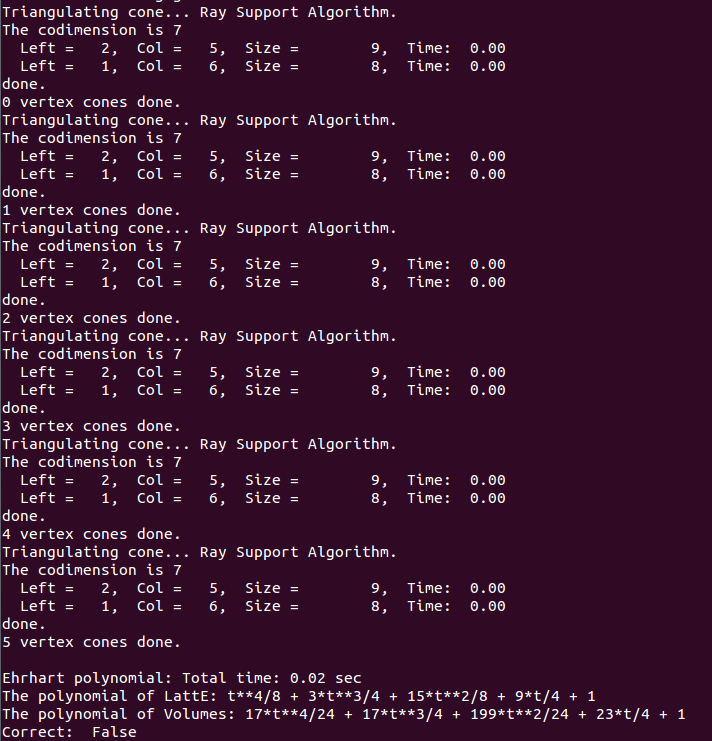
\includegraphics[width=0.35\textwidth]{birk3t8.png}
		\caption{birkhoff polytope birk3.ine t=8}
	\end{figure}

	\item cross polytope d=3 t=5, "lp" \newline
	H-vector: [1, 26, 0, 0] \newline
	Ehrhart polynomial found: (t + 1)*(t + 2)*(9*t + 1)/2 \newline
	\begin{figure}[!h]
  		\centering
         	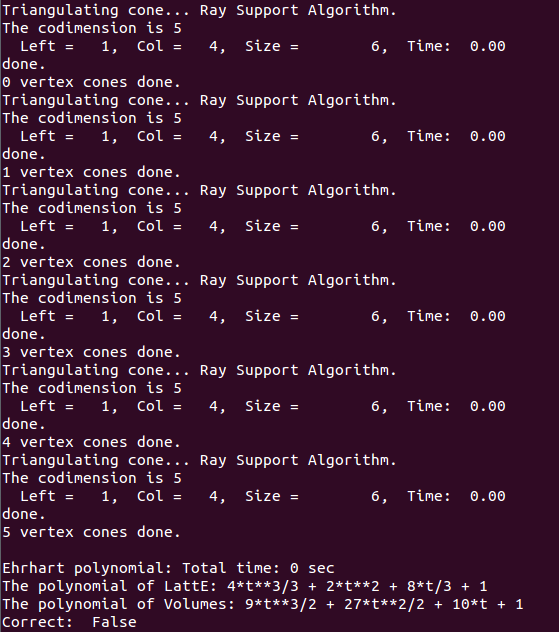
\includegraphics[width=0.32\textwidth]{cross3t5.png}
		\caption{cross polytope cross3.ine t=5}
	\end{figure}	
		
	
\end{itemize}
\newpage
\begin{itemize}


	\item cube polytope d=10 t=11, "lp"
	
	\begin{figure}[!h]
  		\centering
         	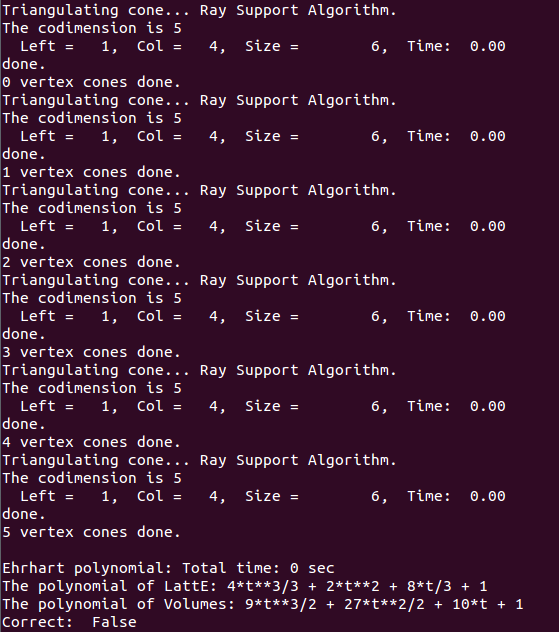
\includegraphics[width=0.50\textwidth]{cross3t5.png}
		\caption{cross polytope cube10.ine t=11}
	\end{figure}	
	
	\item skinny cube polytope d=2 t=3, "lp" \newline
	H-vector: [1, 485, 1] \newline
	Ehrhart polynomial found: (487*t**2 + 487*t + 2)/2 \newline
	
	\begin{figure}[!h]
  		\centering
         	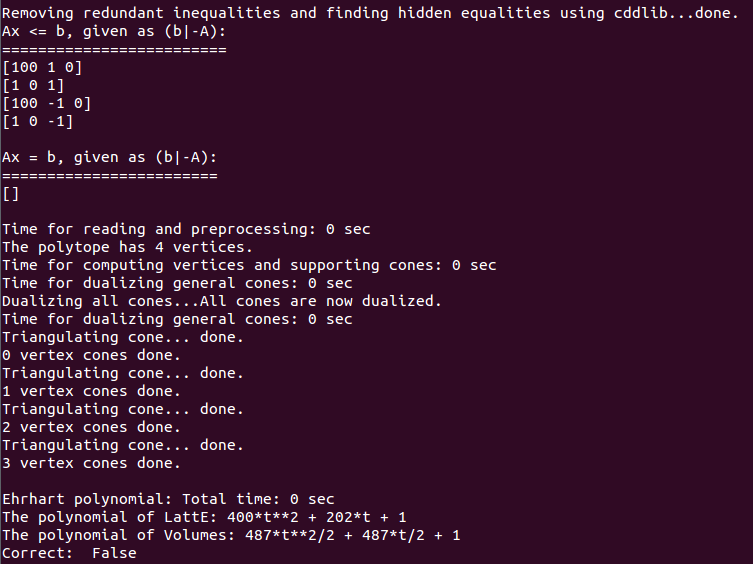
\includegraphics[width=0.50\textwidth]{skinnycube2t3.png}
		\caption{skinny cube polytope for d=2 t=3}
	\end{figure}	
	
	
	\item cross polytope d=2 t=3, "all" \newline
	lattemultipoly:  $t0*t1*t2/((1-t1^(-1)*t2^2)*(1-t2)) + (-1)*t0*t1/((1-t2)*(1-t1^(-1))) + t0*t1*t2/((1-t1^(-1)*t2^2)*(1-t2^(-1))) + t0*t1/((1-t2)*(1-t1^(-1))) + t0*t2^3/((1-t1*t2^(-2))*(1-t2)) + t0*t2^3/((1-t1*t2^(-2))*(1-t2^(-1)))$ \newline
	H-vectors: [[1, 1, 1], [1, 0, 3]] \newline
	Ehrhart candidates: (3*t**2 + 3*t + 2)/2 ,\tab
	2*t**2 + 1 \newline
	Ehrhart polynomial found: 2*t**2 + 1\newline

	\begin{figure}[!h]
  		\centering
         	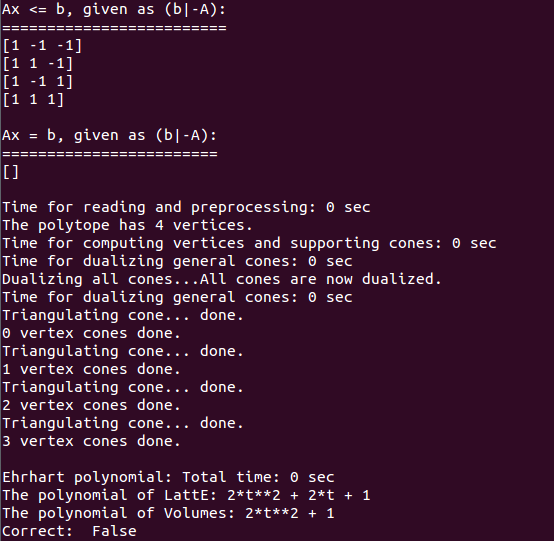
\includegraphics[width=0.50\textwidth]{allcross2t3.png}
		\caption{cross for d=2 t=3}
	\end{figure}	


\end{itemize}

\par
\begin{itemize}
	\item Bigger dimension or dialate values result is not found correctly, It is working forever
	\item Program is finished normally but result is not true because the coefficients have small difference 
	%\item  
\end{itemize}
\newpage
\section{USER MANUEL}
\begin{itemize}
	\item Install the Dokcer into the OS with sudo apt-get install docker.io or
Instructions can be followed from the docker website for installation
	\item  Download the latest version of docker image from the following link to
installation of the necessary tools for project with docker pull
yunusemregtu/bitirme command;
	\begin{itemize}
		\item https://hub.docker.com/r/yunusemregtu/bitirme/
	\end{itemize}	 
	\item Run the docker image with sudo docker run 'imageName'
	\item Download LattE integrale bundle from the following link and extract file to
build file https://www.math.ucdavis.edu/~latte/software.php. Respectively,
give the ./configure prefix=/usr/local and make command on command
line
	\item Clone or Download the python code that calculates the volumes from the
following link: https://github.com/yunusemravci/Volumes-of-Polytopes
	\item Exctract the directory to project file
	\item Give the python Volumes.py polytopeName.ine dilateNumber command
on the command line
\end{itemize}
 \newpage
%\section{REFERENCES}

\addcontentsline{toc}{section}{References}
\begin{thebibliography}{9}
\bibitem{approximation} 
Vissarion Fisikopoulos, Ioannis Emiris 
\\\texttt{https://github.com/vissarion/volume\_approximation}
\textit{The \LaTeX\ Companion}. 
Addison-Wesley, Reading, Massachusetts, 1993.
 
\bibitem{docker} 
What is Docker and Installation steps. 
\\\texttt{https://docs.docker.com/get-started/\#setup}

\bibitem{Ehrhart} 
Ehrhart Theory for Lattice Polytopes,
\\\texttt{http://www.ms.uky.edu/\~braun/Braun\_Dissertation.pdf}

\bibitem{EhrhartPoly} 
Ehrhart Polynomial and Theory,
\\\texttt{https://en.wikipedia.org/wiki/Ehrhart\_polynomial}

\bibitem{convexEhrhart} 
What is convex polytope and relation with Ehrhart Theory,
\\\texttt{https://en.wikipedia.org/wiki/Convex\_polytope}

\bibitem{polytimealg} 
M. Dyer, A. Frieze, and R. Kannan.
[\textit{A random polynomial-time algorithm for
approximat-ing the volume of convex bodies}].
 J. ACM, 38(1):1–17, 1991.



\bibitem{computeVolume} 
M. Dyer, A. Frieze,
[\textit{ On the complexity of computing the volume of a
polyhedron}].
SIAM J. Comput., 17(5):967–974, 1988.


\bibitem{LatticePoint} 
Ehrhart Polynomial and Theory,
\\\texttt{http://www.csie.nuk.edu.tw/\~cychen/Lattices/Sampling\%20lattice\%20points.pdf}

\end{thebibliography}





\newpage
\appendix
%\addcontentsline{toc}{section}{DOCKER FILE SOFTWARE TOOLS}
\section{DOCKER FILE SOFTWARE TOOLS}

	\begin{figure}[!h]
  		\centering
         	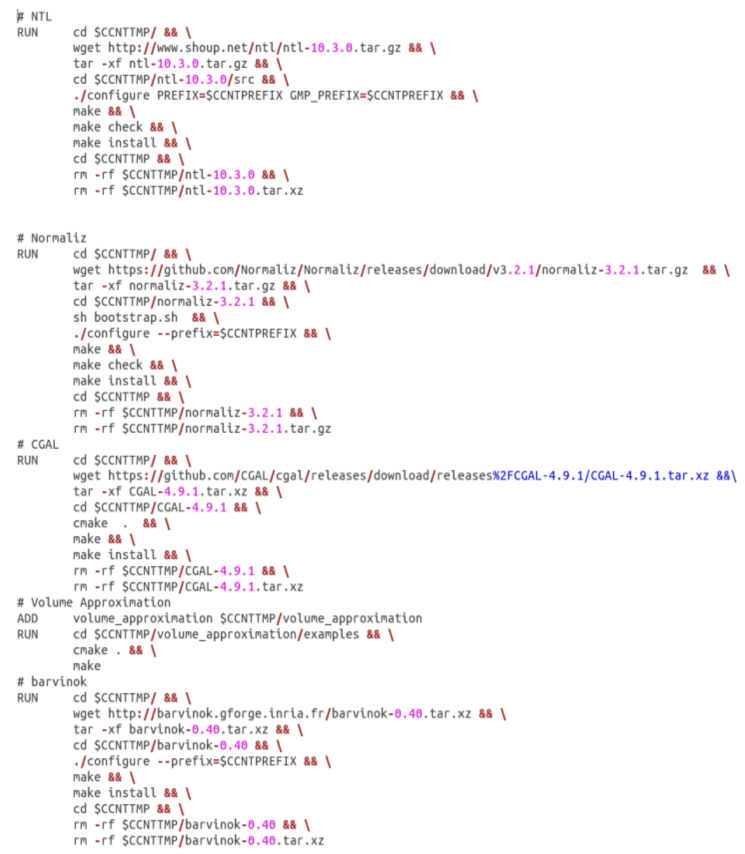
\includegraphics[width=0.90\textwidth]{softtool.png}
		
	\end{figure}	
	
\newpage
%\addcontentsline{toc}{section}{DOCKER FILE SOFTWARE UTILITIES}
\section{DOCKER FILE SOFTWARE UTILITIES}

	\begin{figure}[!h]
  		\centering
         	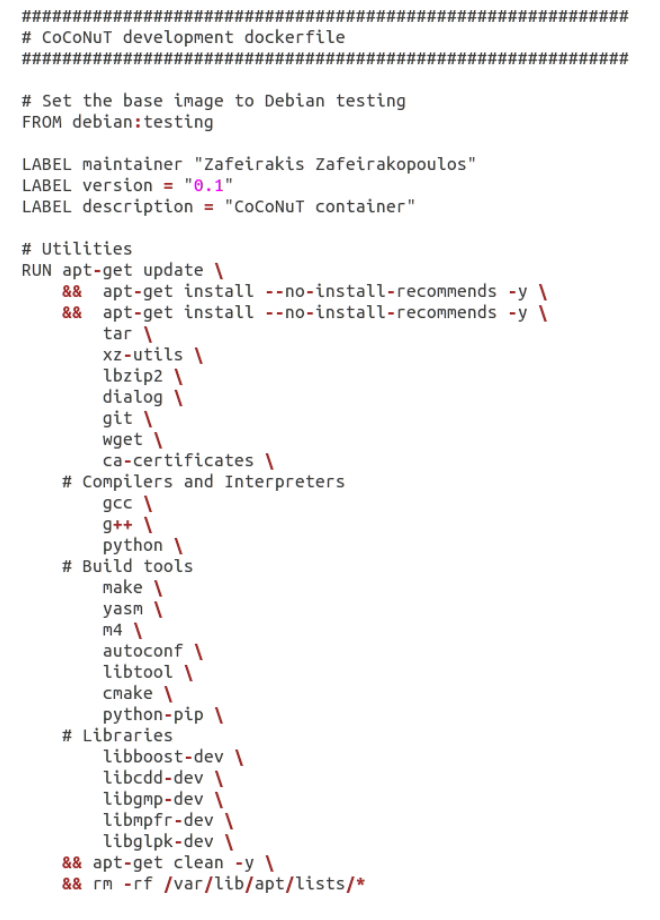
\includegraphics[width=0.90\textwidth]{utilities.png}
		
	\end{figure}	
\newpage
%\addcontentsline{toc}{section}{VOLUMES FOR ONE LATTICE POINT}
\section{VOLUMES FOR ONE LATTICE POINT}

\begin{figure}[!h]
  		\centering
         	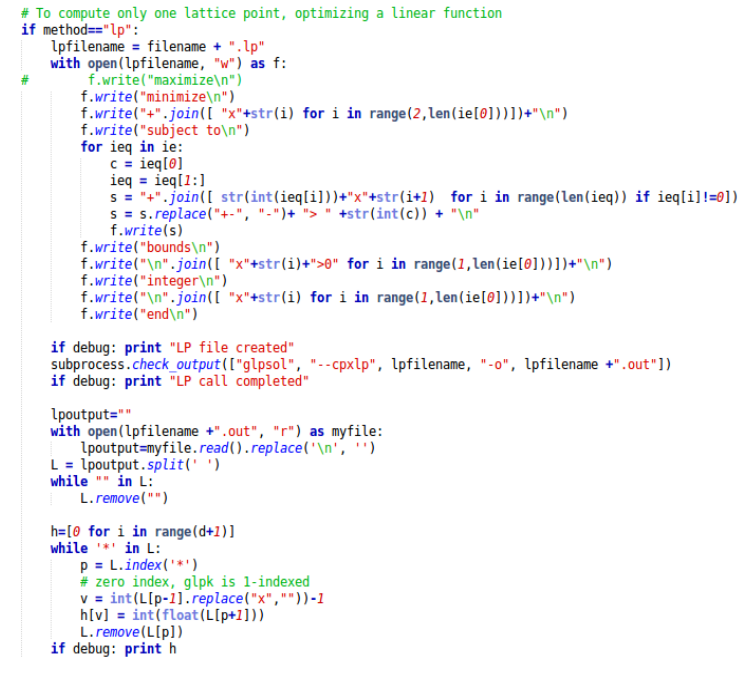
\includegraphics[width=0.90\textwidth]{onelatte.png}
		
	\end{figure}	
\newpage
%\addcontentsline{toc}{section}{VOLUMES FOR ALL CANDIDATES,ALL}
\section{VOLUMES FOR ALL CANDIDATES,ALL}

\begin{figure}[!h]
  		\centering
         	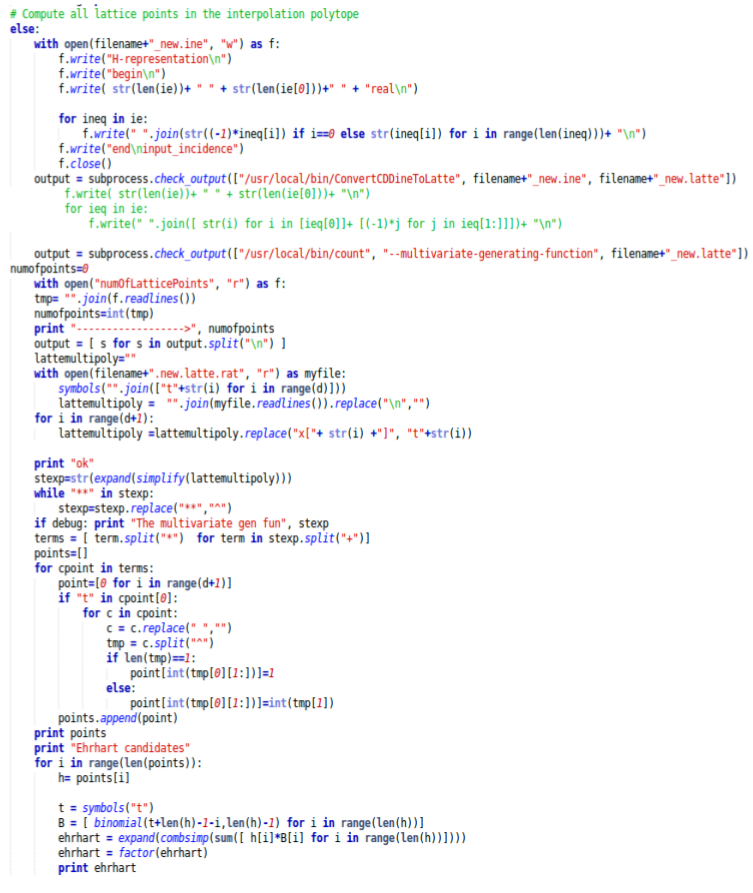
\includegraphics[width=0.90\textwidth]{allLatte.png}
		
	\end{figure}	
\newpage
%\addcontentsline{toc}{section}{DILATE, BOUNDS, INEQUALITIES PART}
\section{DILATE, BOUNDS, INEQUALITIES PART}

\begin{figure}[!h]
  		\centering
         	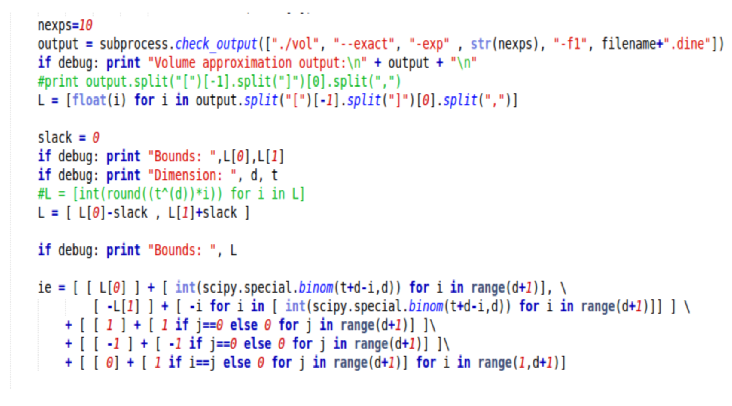
\includegraphics[width=0.95\textwidth]{dilateBounds.png}
		
	\end{figure}	
\end{document}














